\chapter{Hardware Implementation}
\label{Chapter 4}
\lhead{Chapter 4. \emph{Hardware Implementation}}

To help demonstrate the usefulness of the stack in a practical manner, a robot was designed and constructed. This robot, named the \emph{ExplorerBot}, was then used to give a practical reference implementation of a full project utilizing the custom embedded Bluetooth stack in a real-world environment.

\section{Hardware Overview}

The completed robot design for the project contains many useful capabilties for both mobility and exploration. Built on top of a pre-fabricated (including raw DC motors and gearing) "Tank" style hobby robot base, the \emph{ExplorerBot} robot implements the following features:

\begin{itemize}
	\item Primary switch-mode based 5V power supply
	\item Secondary LDO based 3.3V power supply for attached sensors
	\item 2x16 Alphanumeric LCD Screen for feedback to the user
	\item Two momentary pushbuttons for user control
	\item One RGB status LED for basic status feedback
	\item Dual PWM motor control system, with variable speed and direction of DC motors
	\item Level converted I\textsuperscript{2}C bus for the attached sensor(s)
	\item Support for the Atmel \textit{Inertial One} and \textit{Pressure One} sensor boards
	\item High intensity LED based headlights for frontal illumination
	\item Piezo speaker for audio feedback and "horn" like functionality
	\item Atmel \textit{AT90USB1287} 8-Bit Microcontroller
	\item External 128KB SRAM for temporary storage of packets to and from the Bluetooth adapter
\end{itemize}

The complete robot design was created in the \textit{Altium Designer} software, including both the schematic design and board routing. Surface mount components were chosen where possible to reduce the board space required, and two board layers used as this proved to offer the lowest cost/time ratio. The final board design measured 10cm x 15cm, however much of this board space is relatively unused; with optimization, this board space could be reduced considerably.

To get the best results in the construction of the robot, the boards were manufactured commercially. This process ensured the manufactured board's quality while also provided solder mask and silkscreen to reduce the potential for error in the robot's construction.

\section{Hardware Modules}

In the section, the various hardware components of the constructed robot are detailed at the block level. Figure \ref{fig:robotblockhw} below illustrates how the various hardware blocks that comprise the robot connect together to make the final design.

\vspace{1em}

\begin{figure}[H]
	\centering
		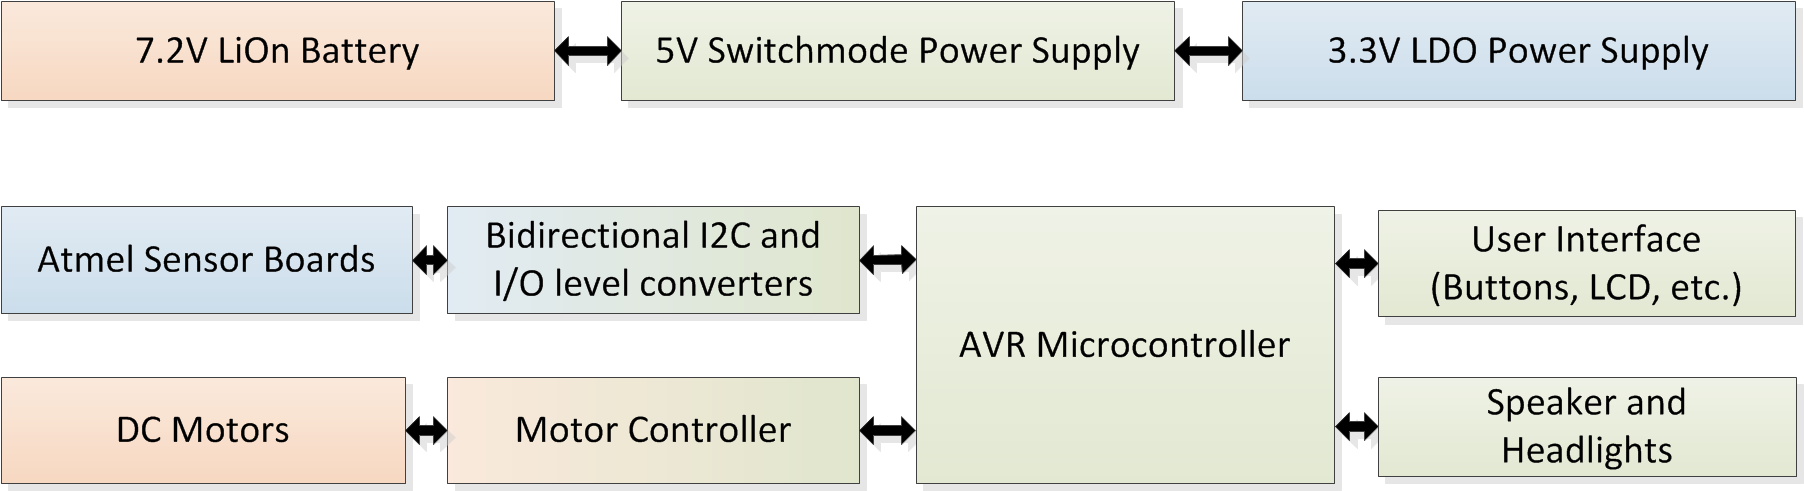
\includegraphics[width=140mm]{./Figures/BlockDiagram.png}
	\rule{35em}{0.5pt}
	\caption[Hardware Block Diagram]{Robot Hardware Block Diagram}
	\label{fig:robotblockhw}
\end{figure}

\subsection{Microprocessor}

Due to the author's familiarity with the Atmel line of \textit{AVR} Microcontrollers, one of the avaliable models in this line-up was chosen to serve in the robot as the main processor, the AT90USB1287. This 8-bit microcontroller contains 128KB of non-voltatile FLASH memory for program storage, 4KB of non-voltatile EEPROM for user application parameter storage and 8KB of internal SRAM for scratch memory. A 16MHz clock (provided by an external crystal) was selected for the design as this offered the fastest possible speed the chip was capable of, while still allowing the hardware USB host controller inside the chip to function normally. As a trade-off, this higher clock speed put a constraint on the main logic level voltage; at 16MHz, the AVR microcontroller requires 5V to be within the datasheet's specifications.

As the AT90USB1287 and associated USB components are difficult to source in single quantities at reasonable prices, the use of a commercial module containing this chip was selected instead: the \textit{Micropendous-A} board (see Figure \ref{fig:micropendous}). This board contains the surface mount AVR microcontroller and associated USB components, along with an external 128KB SRAM chip attached to the AVR's external memory bus interface. As the Bluetooth stack required a large temporary buffer for incoming fragments, the selection of this board proved ideal for the intended purpose.

\begin{figure}
	\centering
		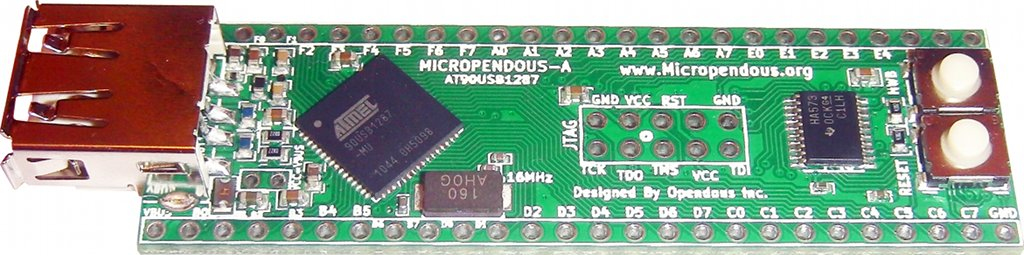
\includegraphics[width=100mm]{./Figures/MicropendousA.jpg}
	\rule{35em}{0.5pt}
	\caption[Micropendous-A Board]{The Micropendous-A Board (Image courtesy \textit{Opendous Inc.})}
	\label{fig:micropendous}
\end{figure}

\subsection{Primary Power Supply}

% TODO

\subsection{User Interface}

% TODO

\subsection{Motor Controller}

% TODO

\subsection{Sensors}

To provide a measure of feedback from the robot, a number of sensors were added to the design. These sensors, when attached, would allow for the robot's environment to be logged and (potentially) reacted to.

\subsubsection{Sensor Power Supply}

While the main system logic and user interface components run from the main switch-mode 5V power supply, the sensor boards were required to run at a fixed 3.3V level, without the possibility of conversion to suit the higher rail voltage.

For this reason, and to reduce the amount of noise on the sensor power supply for maximum precision, a desision was made to add a secondary power supply, running from the 5V rail, to step down the voltage to the 3.3V required by the sensor boards. For maximum noise reduction, a conventonal Low Dropout (LDO) style regular was used.

\subsubsection{Level Converters}

Due to the differing bus voltages between the sensor boards (3.3V) and the main processor (5V), level conversion of the I\textsuperscript{2}C bus and sensor interrupt/control lines was required. While only a unidirectional buffer was strictly needed for each of the sensor interrupt/control lines, it was decided to use a bidirectional converter to ease the board routing.

Initially, only an ADG3308 8-channel Bidirectional Level Converter IC was used, for both the sensor interrupt/control lines, as well as the I\textsuperscript{2}C bus. However, after further analysis it was discovered that the level translater would not meet the timing requirements of the I\textsuperscript{2}C bus, neccesitating the addition of a secondary dedicated TI PCA9306 fixed function I\textsuperscript{2}C bus level converter IC in the second revision of the board. As a bonus, the use of the later chip allowed the I\textsuperscript{2}C bus to be driven at the "Fast" I\textsuperscript{2}C speed of 200KHz for minimal latency and maximum throughput.

\subsubsection{Atmel Sensor Boards}

By designing the robot around the commercially available Atmel sensor boards for sensor feedback, the design of the robot was considerably simplified and the total unit cost lowered. The \textit{Atmel Pressure One} board contains a Bosch BMP085 Pressure Sensor IC for air pressure sensing, while the Atmel \textit{Inertial One} contains a 3-Axis ITG3200 Gyroscope, 3-Axis BMA150 Accelerometer and 3-Axis AK8975 Compass IC. As several of the sensors also contain a digital temperature sensor in addition to the primary sensor (for calibration and stability feedback) this functionality was also used by the robot to measure the environmental temperature in real time.

\begin{figure}
	\centering
		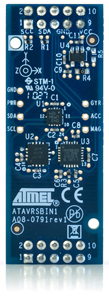
\includegraphics[height=70mm]{./Figures/Inertial1.jpg}
		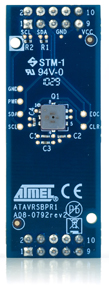
\includegraphics[height=70mm]{./Figures/Pressure1.jpg}
	\rule{35em}{0.5pt}
	\caption[Atmel Sensor Boards]{The Atmel \emph{Inertial One} (left) and \emph{Pressure One} (Right) Sensor Boards (Image courtesy \textit{Atmel Corp.})}
	\label{fig:micropendous}
\end{figure}

